\subsection{Mission Patch}

\includegraphics[width=\textwidth]{logo}
\begin{center}
\textbf{Figure 1: Mission Logo [1]}
\end{center}

\subsection{Project Overview}
The Hephaestus project is a Capstone Senior Design project for Oregon State University's 2016/2017 Senior Design class (CS461-CS463).
The CS senior design project is one part of the overall Hephaestus project.
In addition to the CS team, there is one team of Electrical Engineers and two teams of Mechanical Engineers working on this project through other senior design classes.
The Hephaestus payload is a rocketry payload developed as part of the 2016/2017 RockSat-X program.
The RockSat-X program is a year long program where groups of students develop rocketry payloads with the help of the Colorado Space Grant Consortium and Wallops Flight Facility.
The term "rocketry payload" refers to an experiment inside a section of the rocket.
Each section of the rocket is called a can, and is a standard space that we can fill with an experiment.
The Hephaestus payload shall take up half a can and shall be mounted on a standard base plate provided by Wallops.
We, as the Hephaestus team, will create the hardware and software for the payload, then integrate it into the rocket before launch.

\subsubsection{Project Phases}
The project shall include several phases. The first is the design phase.
The design phase shall last all of Fall 2016 term at OSU.
In the design phase, we shall design the robotics, electronics, materials, and software.
The design phase shall include presentations to the RockSat-X program, where there will review our designs.
Following the design phase will be the implementation phase.
In the implementation phase we shall last through June 2017.
This phase shall include testing of the payload.
We will perform testing both at OSU and at Wallops.
At OSU we will be testing the payload functionality.
At Wallops, we will be testing the structural integrity of the payload, as well as its resistance to vibrations, heat, and cold.
Following the implementation phase will be the integration phase.
This phase will occur at Wallops in July.
This is the point at which our base plate will be integrated into the rocket as a whole, along with the other participating teams.
The final phase will be launch. Launch will occur in Summer of 2017.
The rocket shall be launched from Wallops Flight Facility.
During the flight we shall send telemetry to the ground station at Wallops.
The payload shall perform the experiment once it reaches appogee.
The payload will hopefully be recovered post-flight.

\subsection{Software State Diagram}
\begin{center}
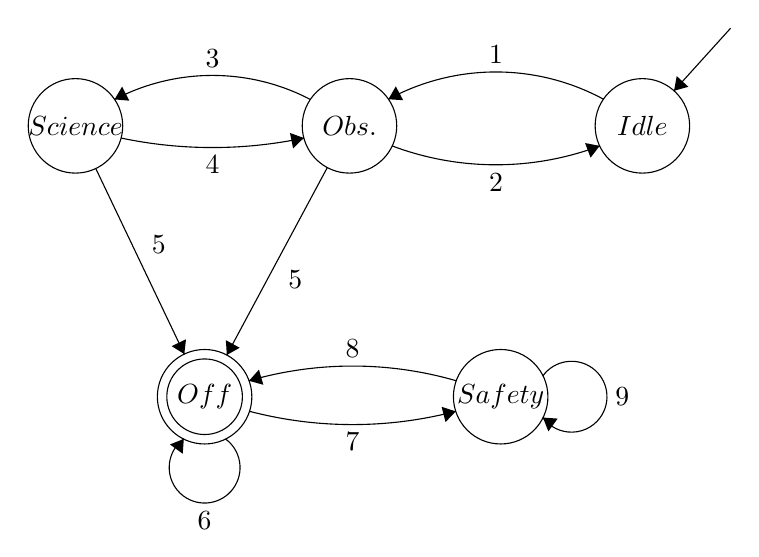
\begin{tikzpicture}[scale=0.2]
\tikzstyle{every node}+=[inner sep=0pt]
\draw [black] (24.2,-19.2) circle (3);
\draw (24.2,-19.2) node {$Obs.$};
\draw [black] (42.8,-19.2) circle (3);
\draw (42.8,-19.2) node {$Idle$};
\draw [black] (6.8,-19.2) circle (3);
\draw (6.8,-19.2) node {$Science$};
\draw [black] (15,-36.4) circle (3);
\draw (15,-36.4) node {$Off$};
\draw [black] (15,-36.4) circle (2.4);
\draw [black] (33.8,-36.4) circle (3);
\draw (33.8,-36.4) node {$Safety$};
\draw [black] (48.4,-13) -- (44.81,-16.97);
\fill [black] (44.81,-16.97) -- (45.72,-16.72) -- (44.98,-16.04);
\draw [black] (26.67,-17.507) arc (118.43354:61.56646:14.344);
\fill [black] (26.67,-17.51) -- (27.61,-17.57) -- (27.14,-16.69);
\draw (33.5,-15.28) node [above] {$1$};
\draw [black] (40.088,-20.475) arc (-69.41442:-110.58558:18.736);
\fill [black] (40.09,-20.47) -- (39.16,-20.29) -- (39.51,-21.22);
\draw (33.5,-22.17) node [below] {$2$};
\draw [black] (9.281,-17.525) arc (117.61533:62.38467:13.416);
\fill [black] (9.28,-17.52) -- (10.22,-17.6) -- (9.76,-16.71);
\draw (15.5,-15.5) node [above] {$3$};
\draw [black] (21.303,-19.973) arc (-78.10445:-101.89555:28.152);
\fill [black] (21.3,-19.97) -- (20.42,-19.65) -- (20.62,-20.63);
\draw (15.5,-21.08) node [below] {$4$};
\draw [black] (8.09,-21.91) -- (13.71,-33.69);
\fill [black] (13.71,-33.69) -- (13.82,-32.75) -- (12.91,-33.19);
\draw (11.61,-26.74) node [right] {$5$};
\draw [black] (16.323,-39.08) arc (54:-234:2.25);
\draw (15,-43.65) node [below] {$6$};
\fill [black] (13.68,-39.08) -- (12.8,-39.43) -- (13.61,-40.02);
\draw [black] (22.79,-21.85) -- (16.41,-33.75);
\fill [black] (16.41,-33.75) -- (17.23,-33.29) -- (16.35,-32.81);
\draw (20.28,-28.97) node [right] {$5$};
\draw [black] (30.948,-37.326) arc (-75.33467:-104.66533:25.865);
\fill [black] (30.95,-37.33) -- (30.05,-37.04) -- (30.3,-38.01);
\draw (24.4,-38.67) node [below] {$7$};
\draw [black] (17.821,-35.385) arc (106.14932:73.85068:23.653);
\fill [black] (17.82,-35.39) -- (18.73,-35.64) -- (18.45,-34.68);
\draw (24.4,-33.95) node [above] {$8$};
\draw [black] (36.48,-35.077) arc (144:-144:2.25);
\draw (41.05,-36.4) node [right] {$9$};
\fill [black] (36.48,-37.72) -- (36.83,-38.6) -- (37.42,-37.79);
\end{tikzpicture}
\end{center}
\begin{center}
Diagram of software states of operation and transition between states.

Transitions between states occur as numbered:

\begin{enumerate}
\item{\textbf{Appogee is reached.} The software shall activate when the power line goes to high at 28V. Observation mode shall be triggered when the OBC turns on.}
\item{\textbf{Error: Return to Idle.} If an error is encountered in entering Observation mode, the software shall fallback to Idle mode and retry. An error may occur if the payload fails to deploy correctly or if the camera fails to turn on.}
\item{\textbf{Payload Assembly and Camera have been deployed.} The software shall enter science mode once the payload assembly and arm have deployed and the camera has performed an observation sweep.}
\item{\textbf{Error: Return to Observation} The software shall return to observation mode if any error occurs in Science mode. An error may occur in Science mode if the arm fails to operate correctly and must return to default position. An error may also occur if the camera stops working.}
\item{\textbf{Timer switches to end appogee period.} Once the time period for observation has ended, the timer line will go to low and trigger to Shutdown state. This state can be reached from either Observation or Science mode.}
\item{\textbf{Accept: Shutdown correctly} If Shutdown occurs correctly, the arm should be closed, the Arm Assembly Body should be retracted, and the OBC should be powered off.}
\item{\textbf{Error: Shutdown not completed successfully.} If an error occurs in the shutdown sequence, the software shall enter Safety mode.}
\item{\textbf{Payload is Shutdown correctly.} If the payload is Shutdown through Safety mode, shutdown can be completed. In Safety mode the payload was either shut down correctly, retracted fully into the can with the arm open, or the arm was expelled safely from the rocket.}
\item{\textbf{Error: Payload is still deployed.} The software shall remain in Safety mode until the payload is either retracted correctly, retracted fully with the arm in the open position, or ejected safely from the rocket. Safety mode shall first try to correctly retract the arm, then retract with the arm open, then repeat attempting ejection until the payload is ejected.}
\end{enumerate}

\subsection{Model of Payload Hardware}
\subsection{Payload Wiring Diagram}
\subsection{References}

\end{document}
\end{center}
